\definecolor{wftext}{RGB}{34,38,45}
\definecolor{wfline}{RGB}{141,118,100}
\definecolor{wffill}{RGB}{252,245,238}
\definecolor{wfdraw}{RGB}{198,132,76}
\definecolor{wfaccent}{RGB}{221,132,59}

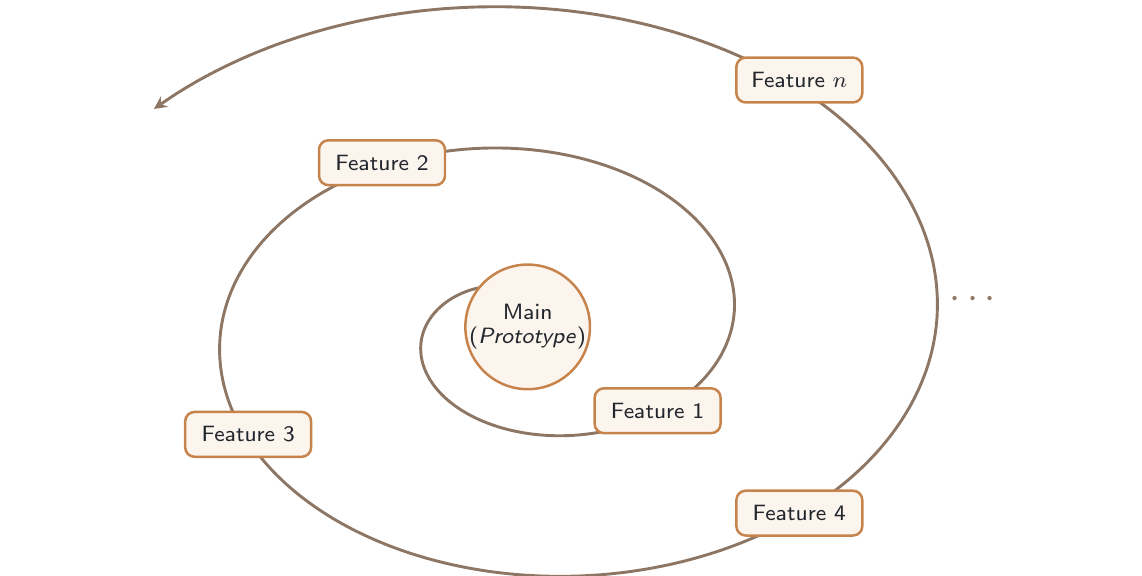
\begin{tikzpicture}[
  x=1cm,
  y=1cm,
  >=stealth,
  every node/.style={inner sep=0pt, outer sep=0pt},
  wfTitle/.style={font=\sffamily\bfseries\fontsize{11}{11.8}\selectfont, text=wftext, align=center},
  wfLabel/.style={font=\sffamily\fontsize{8}{8.6}\selectfont, text=wftext, align=center},
  wfMain/.style={draw=wfline, line width=1.05pt, ->},
  wfConn/.style={draw=wfline, line width=0.9pt},
  wfCore/.style={draw=wfdraw, fill=wffill, line width=0.9pt, circle, minimum size=1.45cm},
  wfBoxA/.style={draw=wfdraw, fill=wffill, rounded corners=0.12cm, line width=0.9pt},
  wfBoxB/.style={draw=wfaccent, fill=wffill, rounded corners=0.12cm, line width=0.9pt}
]

  \path[use as bounding box] (0.8,0.35) rectangle (14.6,6.95);

  \node[wfTitle] at (7.7,7.7) {Spiral schema};

  % Symmetric contained spiral
  \draw[wfMain, samples=220, domain=65:860, smooth, variable=\t]
    plot ({7.15 + (0.0022 + 0.0072*\t)*cos(\t)},
          {3.15 + (0.0022 + 0.0050*\t)*sin(\t)});

  \node[wfCore, wfLabel] (core) at (7.15,3.15) {Main\\(\textit{Prototype})};

  \draw[wfBoxA] (8.00,1.80) rectangle (9.60,2.37);
  \node[wfLabel] at (8.80,2.09) {Feature 1};

  \draw[wfBoxA] (4.50,4.95) rectangle (6.10,5.52);
  \node[wfLabel] at (5.30,5.24) {Feature 2};

  \draw[wfBoxA] (9.80,0.50) rectangle (11.40,1.07);
  \node[wfLabel] at (10.60,0.79) {Feature 4};

  \draw[wfBoxA] (2.80,1.50) rectangle (4.40,2.07);
  \node[wfLabel] at (3.60,1.79) {Feature 3};

  \draw[wfBoxA] (9.80,6.00) rectangle (11.40,6.57);
  \node[wfLabel] at (10.60,6.29) {Feature $n$};

  \node[wfLabel, text=wfline] at (12.80,3.50) {\Large$\cdots$};

\end{tikzpicture}
